% arara: pdflatex
% arara: nomencl
% arara: pdflatex

\documentclass[12pt,letterpaper]{article}
\usepackage{amsmath}
\usepackage[colorlinks]{hyperref} 
\usepackage[title,toc,page]{appendix}
\usepackage{graphicx}
\usepackage{caption}
\usepackage{listings}
\usepackage{titlesec}
\usepackage{todonotes}
\usepackage[intoc]{nomencl}

%% This code creates the groups
% -----------------------------------------
\usepackage{etoolbox}
\renewcommand\nomgroup[1]{%
  \item[\bfseries
  \ifstrequal{#1}{A}{Physics constants}{%
  \ifstrequal{#1}{B}{Transfer Functions}{%
  \ifstrequal{#1}{O}{Other symbols}{}}}%
]}
% -----------------------------------------

\makenomenclature

\renewcommand{\nomname}{List of Symbols}
\renewcommand{\nompreamble}{The following list describes several symbols that will be used later within the body of the document}

\newcommand{\sectionbreak}{\clearpage}

\begin{document}

\title{Oh, What a Bot!}
\author{HackRVA.org}
\date{}
\maketitle

\tableofcontents

\printnomenclature[0.5in]

\section{Introduction}
This article describes the development of a control system model for an reaction wheel pendulum, shown in Figure \ref{sketchOfPendulum}.  A reaction wheel pendulum is a variation of a simple pendulum, balanced upright, with rotating wheels
at the top in place of the pendulum bob. Each wheel is driven by a separate motor.  The pendulum is inherently unstable in the upright position - gravity will pull the pendulum over if it is not perfectly balanced.  Thus, a control system is needed to accelerate the reaction wheels, applying torques
as needed to the pendulum so as to keep it upright. The reaction wheels are mounted at right angles to each other, providing the ability to 
correct the alignment of the pendulum in any direction.

The pendulum physical structure includes a rod, an accelerometer, and two flywheels.  Each
flywheel is comprised of a motor mount, a DC brushed motor, and a reaction wheel.  The flywheel assemblies are mounted at
the top of the rod at right angles to each other and the rod.  The DC motors are wired to a motor controller and an Arduino.  The Arduino is also wired
to the accelerometer, which is located at the top of the rod.

\todo{needs a figure number}The basics of the pendulum control system is outlined in Figure \ref{fig.basicControlSystem}.  The system
can be controlled by adjusting the voltage.  An additional input F is included to describe random environmental forces that may affect the pendulum.  The random forces may result in the desired angle of the pendulum not being achieved.  More accurate control will result from feeding the resulting pendulum angle back into the control system so that the input voltage is continuously adjusted until the desired pendulum angle is achieved.  This is shown in Figure \ref{basicControl}.

In this case, however, the goal is for the pendulum to remain vertical with as little wobble as possible.
The real control comes into play when correcting for the stray forces on the system.  Hence, the control
system can be reformulated as shown in Figure \ref{fig.regulatorControlSystem}, commonly known as
a Regulator Problem.  This structure emphasizes the environmental forces as the primary input into the
system and that the feedback is primarily intended to compensate for those forces.\todo{Figure 3 is missing a feedback arrow}

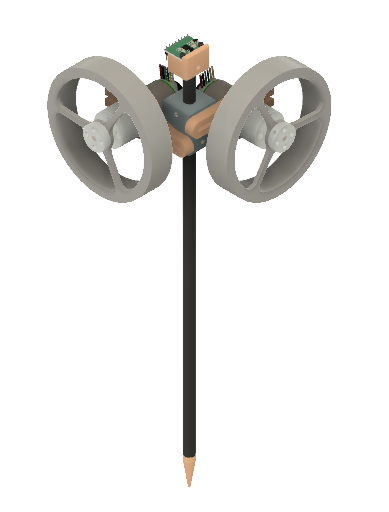
\includegraphics[width=\textwidth]{images/pencil.png} 
    \captionof{figure}{Sketch of the Pendulum}  
    \label{sketchOfPendulum}
   
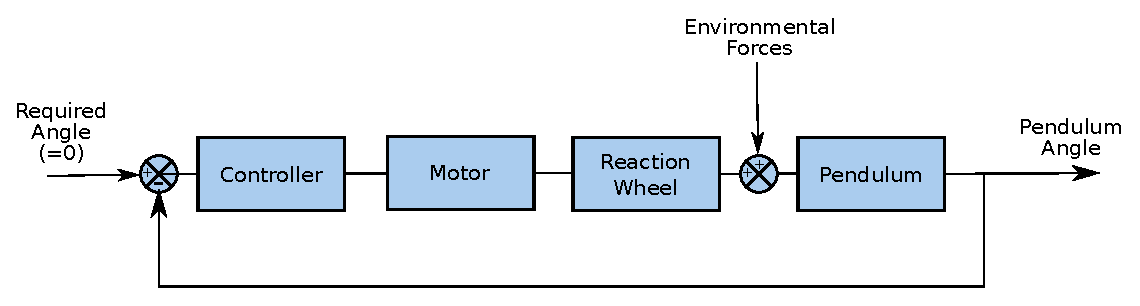
\includegraphics[width=\textwidth]{images/basicControl.eps}
    \captionof{figure}{Simplified Pendulum Model}
    \label{basicControl}

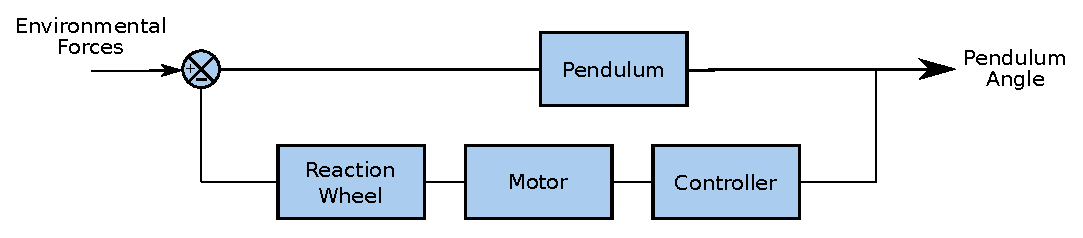
\includegraphics[width=\textwidth]{images/regulator.eps}
    \captionof{figure}{Regulator Model}
    \label{fig.regulatorControlSystem}








\section{Pendulum Dynamics}

More detail can be added to the regulator control system description by building a mathematical model of the the
pendulum.
Figure \ref{modelOfPendulum} shows a simplified sketch of the inverted pendulum.
Reference \cite{reactionWheel} contains a summary of the model dynamics for the balancing pencil.  
The model dynamics can be summarized as
%
\begin{equation}
    m g l \sin \theta + F - I_{c}\ddot{\theta}  = I_{f}\ddot{\phi}
\end{equation}
%

\nomenclature[O]{\(m\)}{total mass of inverted pendulum (kg)}
\nomenclature[A]{\(g\)}{Gravitational constant (m s\textsuperscript{-2})}
\nomenclature[O]{\(l\)}{distance from the pivot point to the center of pendulum mass (m)}
\nomenclature[O]{\(\theta\)}{pendulum angle (rad)}
\nomenclature[O]{\(F\)}{environmental forces on the pendulum}
\nomenclature[O]{\(I_{c}\)}{moment of inertia of the pendulum (kg m\textsuperscript{2})}
\nomenclature[O]{\(I_{f}\)}{moment of inertia of the reaction wheel (kg m\textsuperscript{2})}
\nomenclature[O]{\(\phi\)}{flywheel angle (rad)}

Other references may have alternate formulations using different definitions for $\theta$ and $\phi$.\footnote{Reference \cite{monograph} has a slightly different formulation for the model dynamics; 
the sign of the gravitational term is positive rather than negative.  This difference is caused 
by Reference \cite{monograph} defining the angle from the downward, resting position
while Reference \cite{reactionWheel} defines the angle from the vertical.  
The cosines of angles differing by $\pi$ have opposite signs.}\\


After linearizing the equation by noting that $\sin{\theta} \approx \theta$ for small angles, 
the transfer function for the pendulum is then
%
\begin{equation}
    m \,g \,l \theta + F - I_{c}\ddot{\theta}  = I_{f}\ddot{\phi}
\end{equation}
%
The reaction wheel can be continuously revolving, making the reaction wheel angle $\phi$ less useful as a control parameter.
In its place we will use $\omega = \dot{\phi}$.
%
\begin{equation}
    m \,g \,l \theta + F - I_{c}\ddot{\theta}  = I_{f}\dot{\omega}\label{bigOne}
\end{equation}
%
For ease of use in later analysis, it is beneficial to split \eqref{bigOne} into two parts:
%
\begin{equation}
    m \,g \,l \theta + x(t)   = I_{c}\ddot{\theta}\label{eq.pendulum}
\end{equation}
%
\begin{equation}
    x(t) = F - I_{f}\dot{\omega}\label{eq.oddOne}
\end{equation}
%
\nomenclature[O]{\(x\)}{net torque applied to the pendulum (N m)}
where $x(t)$ is the net torque applied to the pendulum.  The sign convention is important; a positive torque $x(t)$
will accelerate the pendulum in the direction of the positive pendulum angle.  However, the sign convention in 
\eqref{eq.oddOne} indicates that  a positive acceleration of the rotor will result in a \textit{negative} acceleration of the pendulum.

Note that if the pendulum is not vertical (i.e. $\theta = 0$) gravity will begin to pull the pendulum over.  Correcting this requires accelerating the flywheel to apply torque to the pendulum.  A flywheel turning at a constant velocity applies no torque to the pendulum and will not alter the movement of the pendulum.



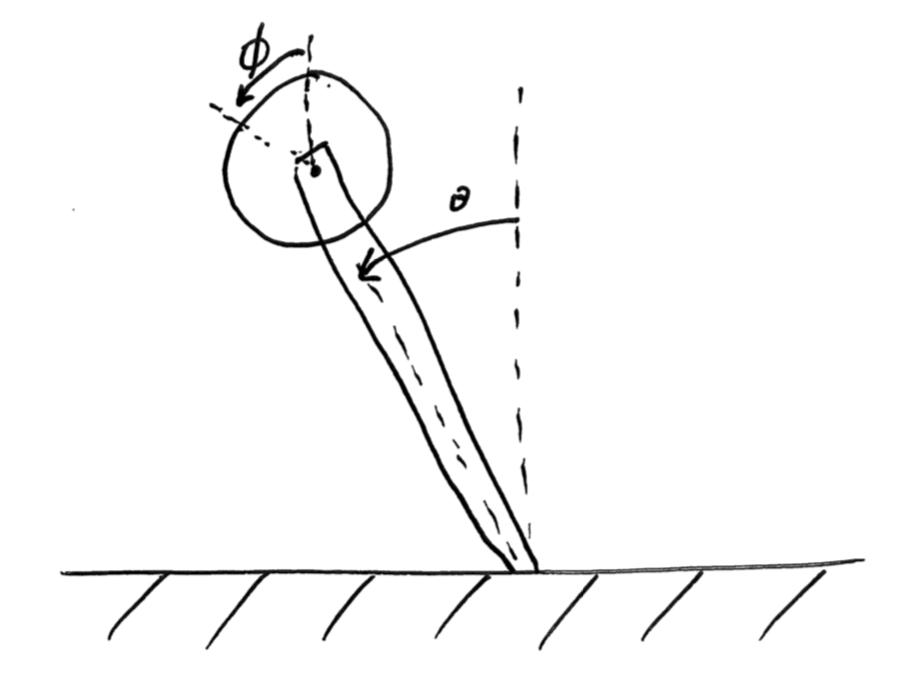
\includegraphics[width=\textwidth]{images/scan1.png}
    \captionof{figure}{Simplified Pendulum Model}
    \label{modelOfPendulum}





\section{Motor and Flywheel Dynamics}

Reference \cite{reactionWheel} models the motor as 
%
\begin{equation}
    I_{f} \, \ddot{\phi} \, \eta_{m} \, \eta_{g}  = K_{t} \, i
\end{equation}
%

\nomenclature[O]{\(\eta_{m}\)}{motor efficiency}
\nomenclature[O]{\(\eta_{g}\)}{gear efficiency}
\nomenclature[O]{\(K_{t}\)}{motor torque constant (N m A\textsuperscript{-1})}
\nomenclature[O]{\(i\)}{motor current (A)}


This formulation appears to have problems, as a reduction in the motor and gear efficiencies results in a 
greater flywheel acceleration for a given motor current.  Similarly, a gear ratio above unity would 
decrease the flywheel acceleration for a specified motor current/torque, which is non-physical.  The equation can be altered
to correct these issues, resulting in the following:
%
\begin{equation}
	I_{f} \, \ddot{\phi} = \, \eta_{m} \, \eta_{g} K_{t} \, i
\end{equation}
%
However, this format may not be the easiest to implement, as the motor and gear efficiencies are not known.  Reference \cite{monograph}
takes a different approach,\footnote{Note that there is no term in \eqref{simpleShaft} that represents torque associated
with external work done by the shaft.  Hence this formulation is limited to flywheels that are reasonably aerodynamic (e.g. not something that
acts as a propeller).}
%
\begin{equation}
    I_{f} \, \ddot{\phi} = T_{shaft}\label{simpleShaft}
\end{equation}
%
Where the earlier format dealt with motor/gear efficiencies using $\eta_{m}$ and $\eta_{g}$, Reference \cite{monograph} develops a correlation of friction in terms of torque required to maintain a given $\dot{\phi}$.  Here the torque will be
reformulated as 
%
\begin{equation}
    T_{shaft} = T - T_{friction}
\end{equation}
%
\begin{equation}
    T_{friction} = A \, sgn(\dot{\phi} - \dot{\theta} ) + B (\dot{\phi} - \dot{\theta})
\end{equation}
%
\begin{equation}
    T = K_{t} \, i
\end{equation}
%

\nomenclature[O]{\(T\)}{total motor torque (N m)}
\nomenclature[O]{\(T_{shaft}\)}{torque available to the flywheel (N m)}
\nomenclature[O]{\(T_{friction}\)}{torque lost to motor and gear friction (N m)}
\nomenclature[O]{\(A\)}{coulomb friction coefficient (N m)}
\nomenclature[O]{\(B\)}{rotational friction coefficient(N m rad\textsuperscript{-1} s)}

Note the use of $(\dot{\phi} - \dot{\theta})$.  Friction is dependent on the relative motion of the motor armature and the motor frame.  If the pendulum angular velocity $\dot{\phi}$ is equal to the reaction wheel angular velocity $\dot{\theta}$ there will be no relative motion between the motor armature and frame; no friction will occur.

Combining equations,
%
\begin{equation}
    I_{f} \, \ddot{\phi}  = K_{t} \, i - A \, sgn(\dot{\phi} - \dot{\theta} ) - B (\dot{\phi} - \dot{\theta})
\end{equation}
%
Again, using the notation $\omega = \dot{\phi}$,
%
\begin{equation}
    I_{f} \, \dot{\omega}  = K_{t} \, i - A \, sgn(\omega - \dot{\theta}) - B (\omega - \dot{\theta}) \label{wheel}
\end{equation}
%

As will be seen, this equation is easier to implement because $K_{t}$, $A$, and $B$ can be measured experimentally (see Appendix \ref{appendix:measure}).  







\section{Motor Control}
The previous chapter determined the relationship between the motor current and the acceleration of the flywheel.  
However, the motor will be not be controlled via motor current.  Instead, a motor controller will be used to control the 
motor by adjusting the motor voltage via a PWM signal.  The equivalent, average voltage will then regulate the motor.  
Following Reference \cite{monograph}, but recognizing the motor is at the end of a pendulum, the relationship between motor current and voltage is
%
\begin{equation}
    L\, \frac{di}{dt} + r \,i = v - K_{v} \, (\omega - \dot{\theta})
\end{equation}
%

\nomenclature[O]{\(L\)}{armature inductance (H)}
\nomenclature[O]{\(r\)}{armature resistance ($\Omega$)}
\nomenclature[O]{\(v\)}{voltage supplied to the motor (V) }
\nomenclature[O]{\(K_{v}\)}{motor voltage constant (V rad\textsuperscript{-1} s)}
\nomenclature[O]{\(\omega\)}{motor rotation speed (rad s\textsuperscript{-1})}

Normally the inductance of the motor is much lower than the resistance, such that $L/r \sim 0.001$ sec.  
In such cases it is acceptable to ignore the time dependence of the current and write
%
\begin{equation}
    r \,i = v - K_{v} \, (\omega - \dot{\theta}) \label{motor}
\end{equation}
%

Solving for i:
%
\begin{equation}
    i = \frac{v}{r} - \frac{K_{v} \, (\omega - \dot{\theta})}{r}
\end{equation}
%
Combining with \eqref{wheel}
%
\begin{equation}
    I_{f} \, \dot{\omega}  =  K_{t} \, \left( \frac{v}{r} - \frac{ K_{v} \, (\omega - \dot{\theta})}{r} \right) - A \, sgn(\omega - \dot{\theta} ) - B (\omega - \dot{\theta})
\end{equation}
Rearranging,

\begin{equation}
    I_{f} \, \dot{\omega} + \left( B+\frac{K_{t} K_{v}}{r} \right) (\omega - \dot{\theta}) +A \, sgn(\omega - \dot{\theta})= \left(\frac{K_{t}} {r}\right)v \label{eq.motorSemiFinal}
\end{equation}

Not all of the voltage results in acceleration of the reaction wheel.  As the reaction wheel velocity increases, an
increasing amount of the voltage (and the resulting torque) is consumed by friction and the back EMF.\\

The voltage used to drive the motor is determined by the controller.  Here the voltage will be set to the output of the controller
\begin{equation}
    v = u 
\end{equation}
\nomenclature[O]{\(u\)}{controller output}
Substituting into \eqref{eq.motorSemiFinal}
\begin{equation}
    I_{f} \, \dot{\omega} + \left( B+\frac{K_{v} K_{t}}{r} \right) (\omega - \dot{\theta}) +A \, sgn(\omega - \dot{\theta}) = \left(\frac{K_{t}} {r}\right)u\
\end{equation}
The simple substitution of $u$ for $v$ does not seem to have much purpose at this point in the analysis, but will be useful
when complex controllers are evaluated.\\

It is useful to assume that the control function can adjust the demand voltage by adding or subtracting a constant, depending on the current spin direction of the reaction wheel.  This means that $-A\,sgn(\dot{\phi})$ is folded
into $u$ for the purposes of this analysis.  Our motor control equation is then
\begin{equation}
    I_{f} \, \dot{\omega} + \left( B+\frac{K_{v} K_{v}}{r} \right) (\omega - \dot{\theta}) = \left(\frac{K_{t}} {r}\right)u\label{eq.motorFinal} 
\end{equation}










\section{Modeling in the Frequency Domain}
\label{sec:Modeling}

The primary objectives of a control system for the pendulum should be to stabilize the upright position of the pendulum and recovering from external forces on the pendulum.  In addition, the control system should be designed to deal with a number
of physical limitations of the physical components of the pendulum.  Specifically,
\begin{itemize}
    \item the motor voltage is limited to maximum value,
    \item the rotor velocity has a practical upper limit.
\end{itemize}


The stability of the system shown in Figure  \ref{fig.regulatorControlSystem} can be evaluated by examining the
open loop transfer function
\begin{equation}
    T(s) = P(s) C(s) M(s) R(s)
\end{equation}

\nomenclature[B]{\(P(s)\)}{pendulum transfer function}
\nomenclature[B]{\(C(s)\)}{control function}
\nomenclature[B]{\(M(s)\)}{motor transfer function}
\nomenclature[B]{\(R(s)\)}{rotor transfer function}
\nomenclature[B]{\(T(s)\)}{open loop transfer function}


The control system in terms of these transfer functions is shown in Figure \ref{transferFunction}.\\


The controller, at this point in the analysis, is assumed to be a pass-through, or
%
\begin{equation}
u = \theta
\end{equation}
Hence, the controller transfer function is
\begin{equation}
C(s) = \frac{u(s)}{\theta(s)} = 1
    \label{EQ.simpleController}
\end{equation}

The pendulum transfer function can be derived from \eqref{eq.pendulum}
%
\begin{equation}
    m \,g \,l \theta(s) + x(s) = I_{c}\theta(s) s^{2}
\end{equation}

Ignoring the environmental forces, the pendulum transfer function is 
\begin{equation}
    P(s) = \frac{\theta(s)}{x(s)}= \frac{1}{I_{c} s^{2} - m g l }
    \label{franco}
\end{equation}
%
The rotor transfer function can be derived from \eqref{eq.oddOne} by noting that the torque generated by the flywheel is
\begin{equation}
    x(s) = F(s) - I_{f}\omega(s) s
\end{equation}
%
\begin{equation}
    R(s) = \frac{x(s)}{\omega(s)} = -I_{f} s
    \label{groucho}
\end{equation}\\

Note that the transfer function for the rotor in \eqref{groucho} is negative.  Combined with the summing
junction shown in Figure \ref{transferFunction}, this produces a negative feedback control system.\\
 


The motor transfer function must be derived from \eqref{eq.motorFinal}.  However,  in \eqref{eq.motorFinal} $\omega$
is a function of both $\theta$ and $u$, preventing the determination of a single-input, single-output transfer function.  One solution is to make the approximation $\omega \approx (\omega - \dot{\theta})$.  The reaction wheel may rotate at hundreds of RPM, while the pendulum is expected to deviate from vertical for only brief periods.  With this approximation 
the motor transfer function can be derived from \eqref{eq.motorFinal} as
\begin{equation}
    I_{f} \, \omega(s) s + \left( B+\frac{K_{v} K_{t}}{r} \right) \omega(s) = \left(\frac{K_{t}} {r}\right)u(s)
\end{equation}
%
\begin{equation}
    M(s) = \frac{\omega(s)}{u(s)} =  \frac{\left(\frac{K_{t}} {r}\right)}{I_{f} s + (\frac{K_{v} K_{t}}{r}+B)}
    \label{rondo}
\end{equation} 

Using \eqref{EQ.simpleController}, \eqref{franco}, \eqref{groucho}, and \eqref{rondo} results in 
%
\begin{equation}
	T(s) =\frac{-(\frac{1} {I_{c}})(\frac{K_{t}}{r})s}
	{(s^2-\frac{m g l}{I_{c}})(s+(\frac{K_{v} K_{t}}{r I_{f}}+\frac{B}{I_{f}}))}
\end{equation}

Substituting in values from the appendixes, the transfer function for the pendulum is
\begin{equation}
	T(s) =\frac{-0.1731 s}{s^3 + 3.113 s^2 -34.8 s -108.3}
\end{equation}

The numerator of the transfer function is the characteristic equation that, when factored, is
$(s-5.899) (s+5.899) (s+3.113)$.

Using the root locus technique and the open loop transfer function, Figure \ref{rootLocus} shows the
behavior of the closed loop poles as a function of feedback gain.  Note that one pole is always in the right
half of the plane, indicating that the system is unstable regardless of the magnitude of the gain. \\


The system might be stabilized by using both proportional and derivative, or PD, feedback.  The control function would be:
\begin{equation}
	u = \theta + p\dot{\theta}
\end{equation}
thus
\begin{equation}
	C(s) = 1 + p s
\end{equation}
Rearranging,
\begin{equation}
	C(s) = p\left(s+\frac{1}{p}\right)\label{pd}
\end{equation}

indicating a zero at $1/p$ and a gain of $p$.
The results are sensitive to the placement of the zero.  Placing the zero to the right of the pole at -5.8993 
eliminates any oscillation but does not remediate the pole in the right half of the plane.  Placing the zero to the left of the pole at -5.8993 results in a much faster response but can result in oscillations (Figure \ref{rootLocusPD}).  Again, the pole in the right half of the plane is not remediated. \\


One additional possibility for resolving the issue of the zero at the origin would be to implement a PID controller.
\begin{equation*}
	u(t) = \theta(t) + q\int \theta\,dt + p\dot{\theta}
\end{equation*}
then
\begin{equation}
	C(s) = 1 + \frac{q}{s} + p s
\end{equation}
Rearranging,
\begin{equation}
	C(s) = p\left(\frac{s^2+\frac{s}{p}+\frac{q}{p}}{s}\right)
\end{equation}

This controller would have two zeros that can be placed as required and a pole that would cancel
the zero at the origin.  If the zeros are placed to the left of the pole at -4.7303, then the system may stabilize.
However, in the real world the original zero may not be exactly at the origin and the poles in the left side of the axis may not be exactly where they are expected (due to nonlinearities, etc.) 
leading to a less-than robust control system. \todo{verify this}\\

Finally, it is possible to include feedback from the other monitored and controlled variable, the rotor velocity.
Unfortunately, to continue to evaluate the system using a root locus analysis, the feedback from
the rotor velocity cannot be included directly in $C(s)$, as it would introduce a second input into the transfer function.  
Instead, the definition of the motor voltage $v$ is modified to include the effect of the rotor velocity feedback
\begin{equation}
    v = u + K_{\omega}\omega
\end{equation}
\nomenclature[O]{\(K_{\omega}\)}{rotor velocity feedback gain}

where $u$ continues to represent the output of a PID controller using $\theta$ as an input and $K_{\omega}\omega$ is an additional feedback
from the rotor velocity.
%
This results in \eqref{eq.motorFinal} transforming into
\begin{equation}
    I_{f} \, \dot{\omega} + \left( B+\frac{K_{v}^2}{r} \right) \omega +A \, sgn(\omega)= \left(\frac{K_{v}} {r}\right)(u + K_{\omega}\omega)
\end{equation}
The motor transfer function is then
\begin{equation}
    I_{f} \, \omega(s) s + \left( B+\frac{K_{v}^2}{r} \right) \omega(s) = \left(\frac{K_{v}} {r}\right)(u(s)+K_{\omega} \omega(s))
\end{equation}
Rearranging terms,
\begin{equation}
    M(s) = \frac{\omega(s)}{u(s)} =  \frac{\left(\frac{K_{v}} {I_{f}r}\right)}{s + (\frac{1}{I_{f}})(\frac{K_{v}^2}{r}-\frac{K_{v} K_{\omega}}{r}+B)}
    \label{rondoMucho}
\end{equation} 

Using \eqref{pd}, \eqref{franco}, \eqref{groucho}, and \eqref{rondoMucho}, the open loop transfer function is now
\begin{equation}
	T(s) =\frac{-(\frac{Kp} {I_{c}r})(s+\frac{1}{p})s}
	{s^3 + (\frac{B r-K K_{\omega}+K^2}{I_{f}r})s^2 - (\frac{m g l}{I_{c}})s - (\frac{Br-K K_{\omega}+K^2}{I_{f}r} - \frac{m g l}{I_{c}})}\label{eq.openLoop}
\end{equation}

Figure \ref{rootLocusFull} shows the root locus with $p = 1/4.5$ and $K_{\omega} = 0.075$.  With a controller gain\footnote{The gain given here is in addition to the system gain modeled in \eqref{eq.openLoop}. } of 370 the controlling close loop poles are at -11.3, -1.33, and -1.12.\\

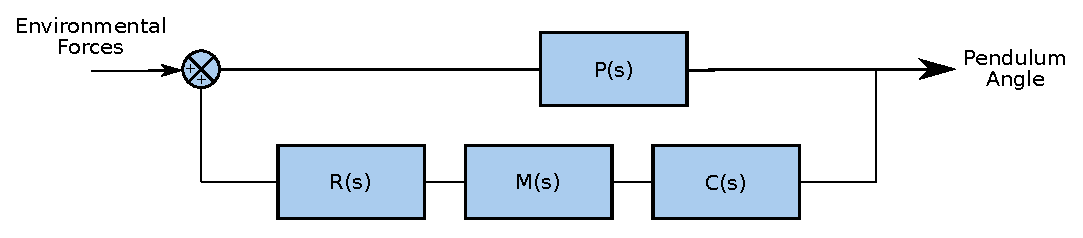
\includegraphics[width=\textwidth]{images/transferFunction.eps}
    \captionof{figure}{Control System Modeled as Transfer Functions}
    \label{transferFunction}

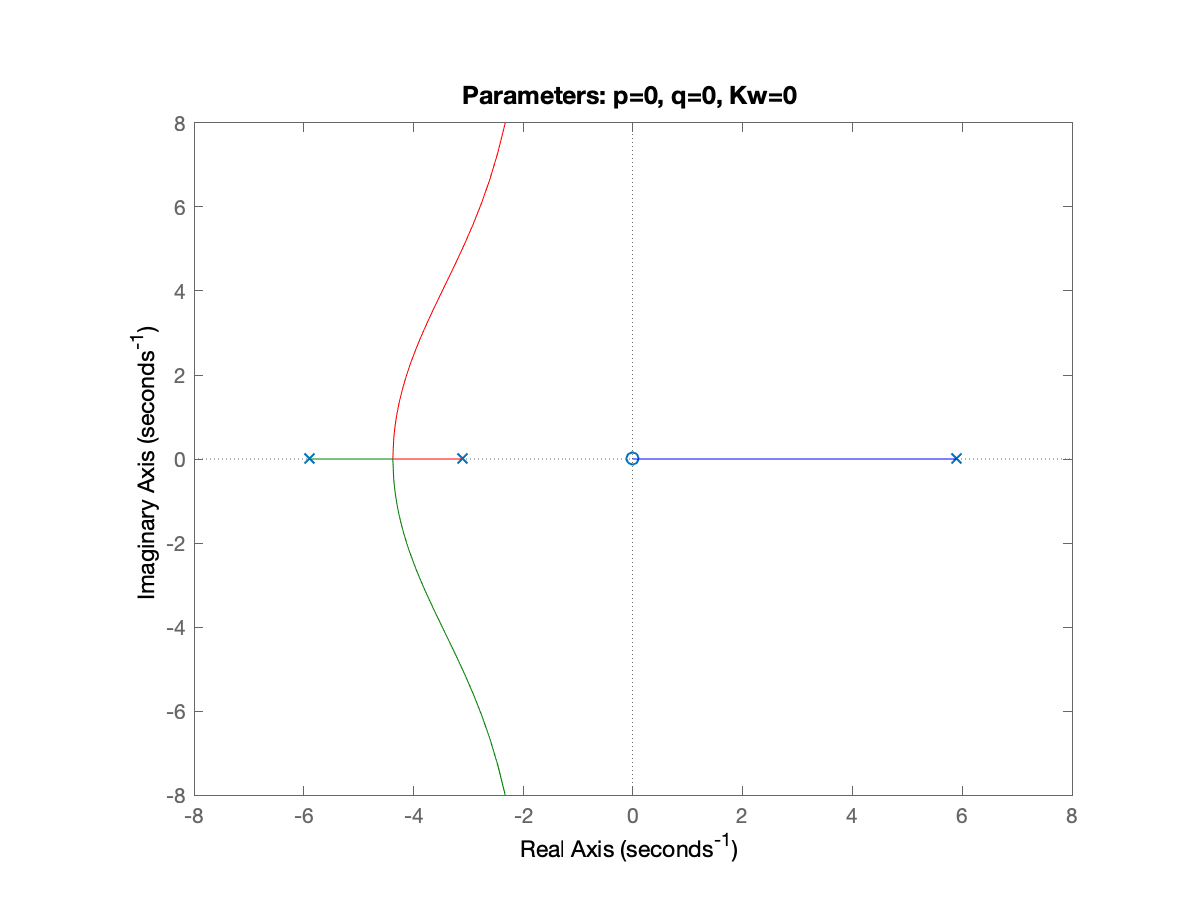
\includegraphics[width=\textwidth]{images/rootLocus.eps} 
    \captionof{figure}{Root Locus Plot With Proportional Feedback}  
    \label{rootLocus}

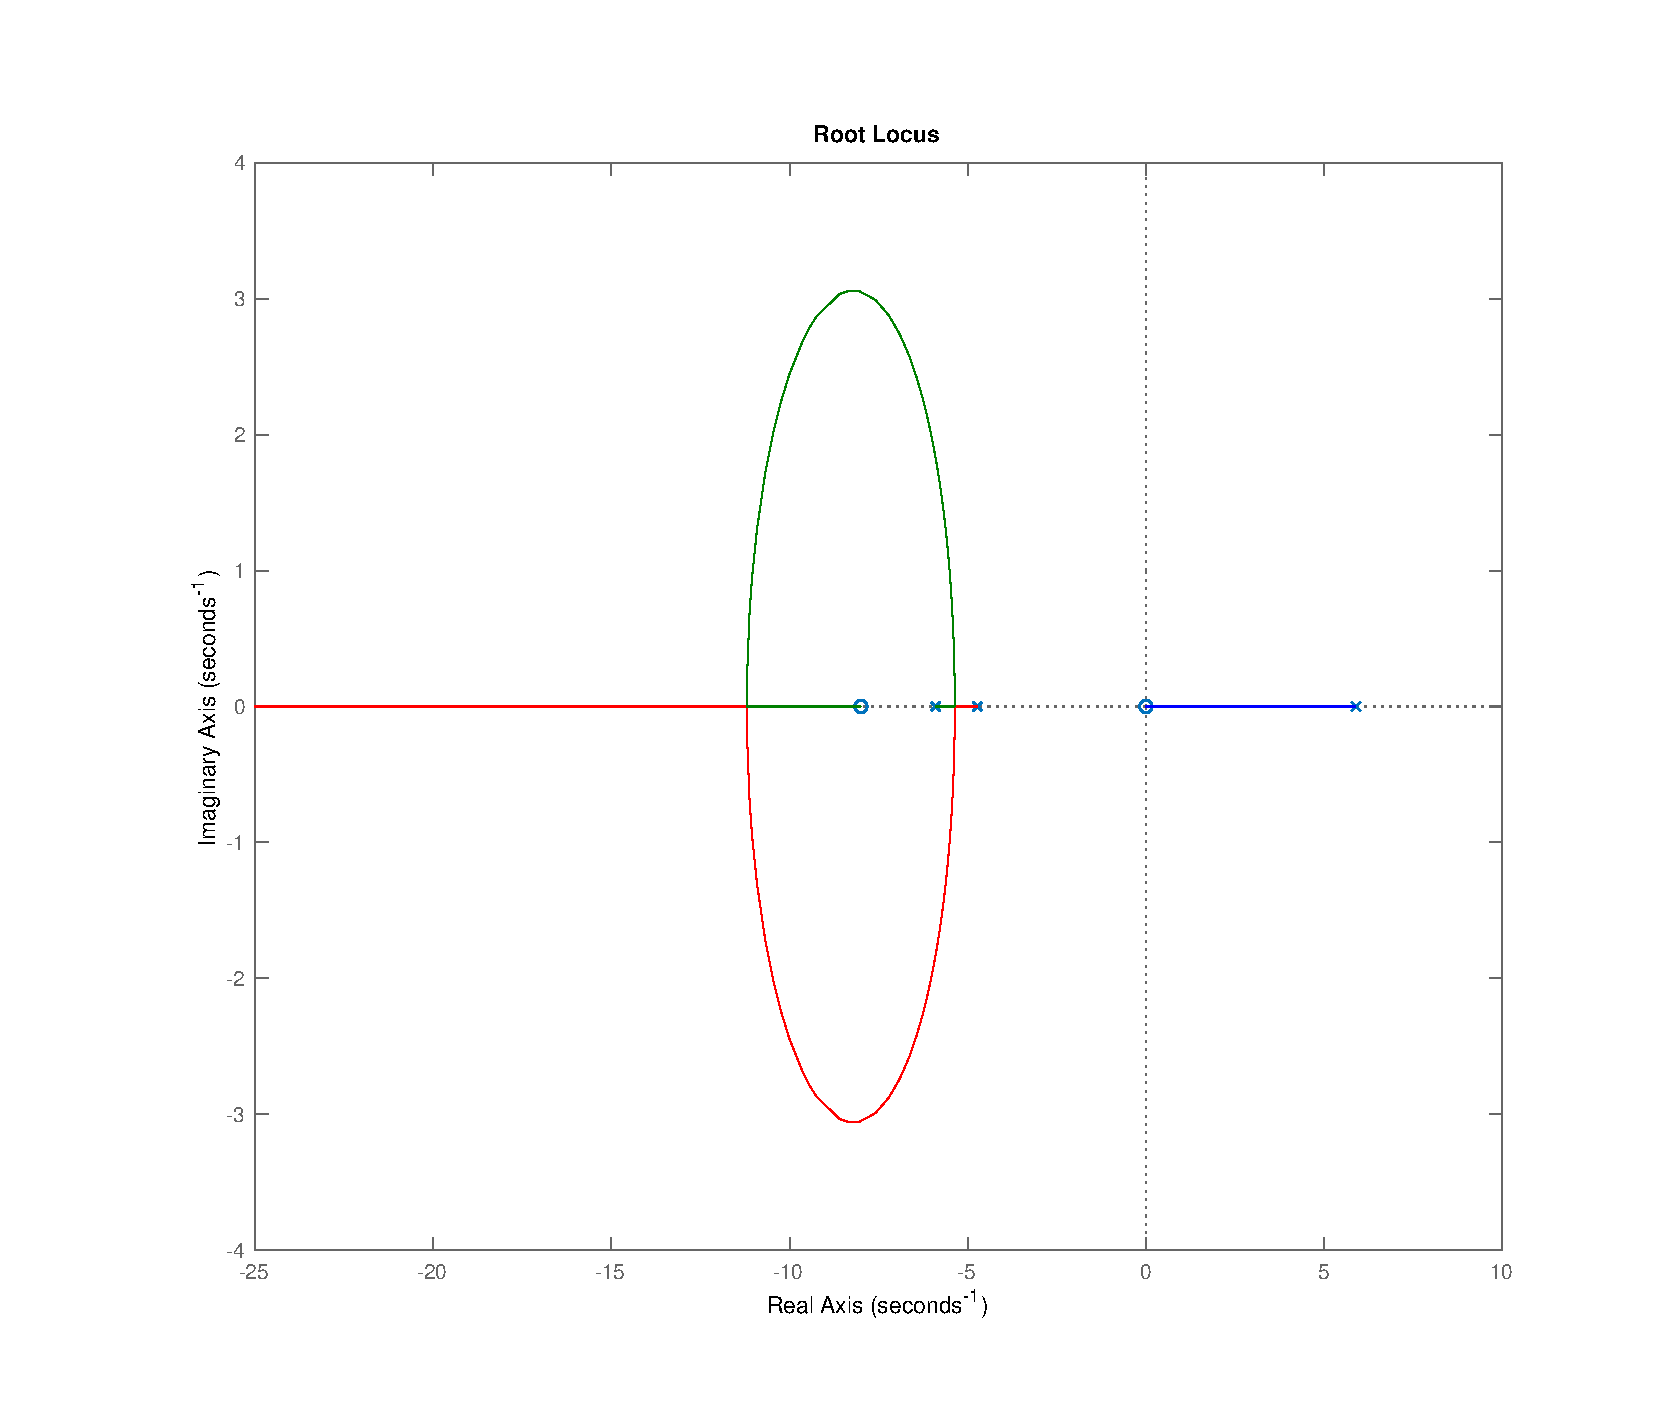
\includegraphics[width=\textwidth]{images/rootLocusPD.eps} 
    \captionof{figure}{Root Locus Plot With PD Feedback}  
    \label{rootLocusPD}

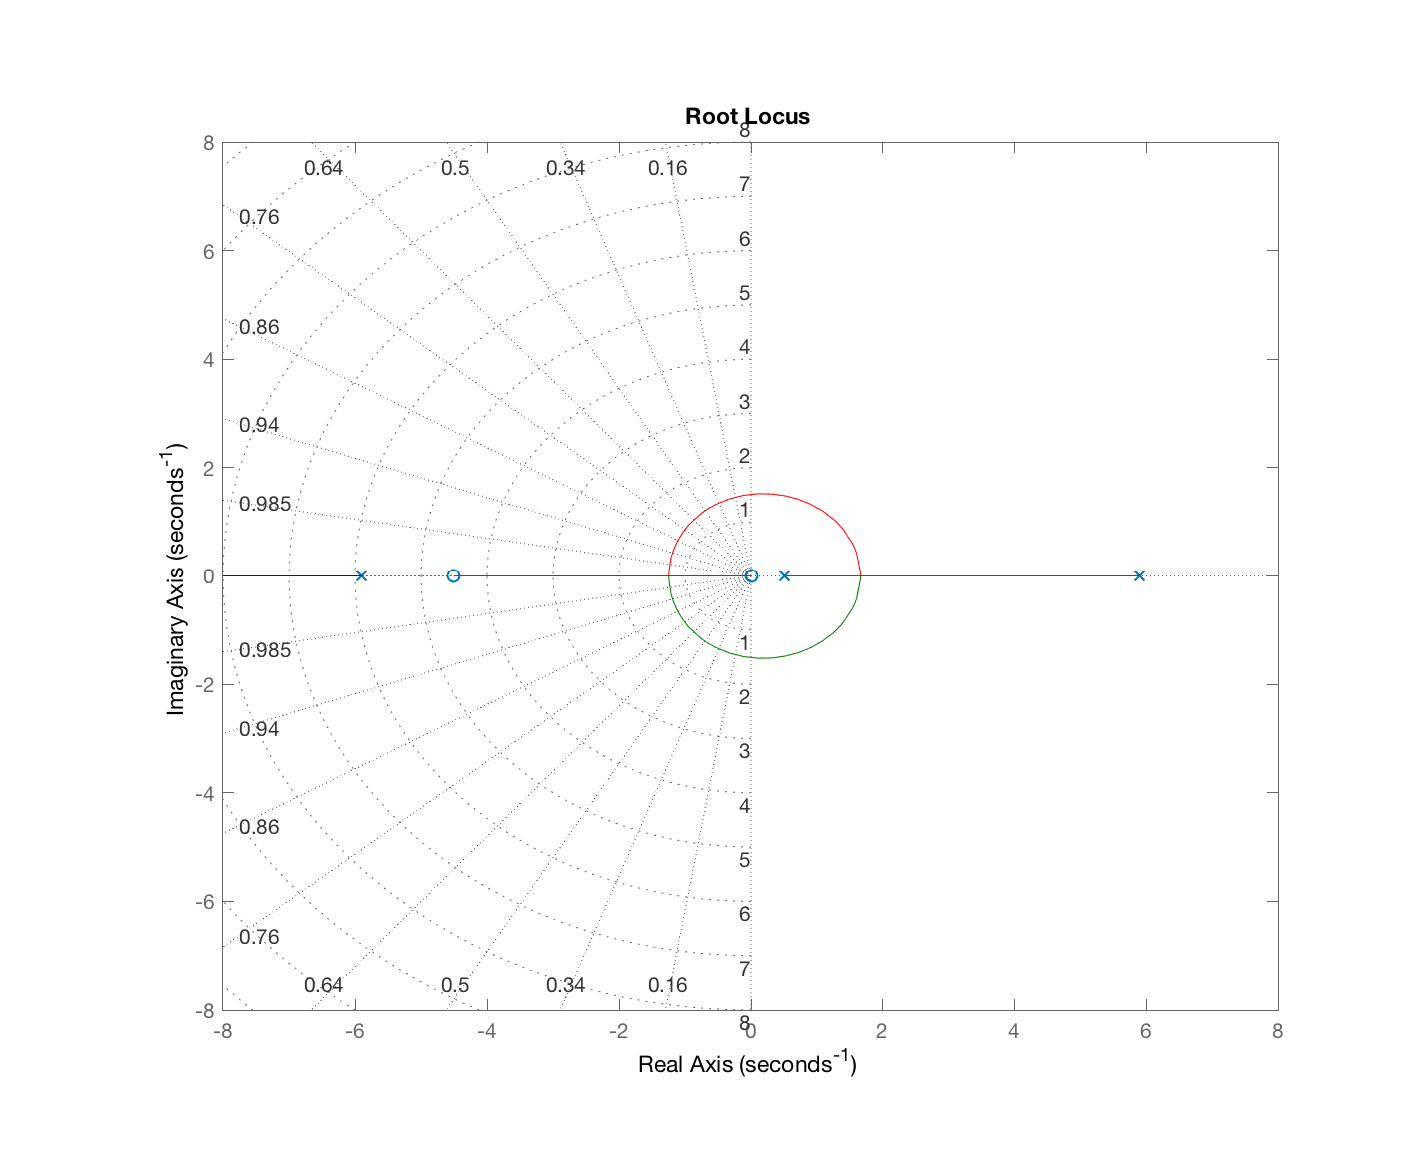
\includegraphics[width=\textwidth]{images/rootLocusFull.eps} 
    \captionof{figure}{Root Locus Plot With PD and Rotor Velocity Feedback}  
    \label{rootLocusFull}

\section{State Space Model}

A State Space model can be constructed from equations \eqref{eq.motorSemiFinal} and \eqref{bigOne}.  The
state space variables are $\omega$, $\theta$, and $\dot{\theta}$.  The state space model
is then
\begin{equation}
\dot{x_{m}} = A_{m} x + B_{m} v
\end{equation}
where $x_{m} = (\omega, \theta, \dot{\theta})^{T}$ and

\begin{equation}
A_{m} = 
\begin{bmatrix}
-\frac{B}{I_{f}}-\frac{K_{v} K{t}}{I_{f} r} & 0 & \frac{B}{I_{f}}+\frac{K_{v} K{t}}{I_{f} r}\\
0 & 0 & 1\\
\frac{B}{I_{c}}+\frac{K_{v} K{t}}{I_{c} r} & \frac{mgl}{I_{c}} & -\frac{B}{I_{c}}-\frac{K_{v} K{t}}{I_{c} r}
\end{bmatrix}
\end{equation}

\begin{equation}
B_{m} = 
\begin{bmatrix}
\frac{K_{t}}{I_{f} r} \\
0 \\
 -\frac{K_{t}}{I_{c} r}
\end{bmatrix}
\end{equation}

However, measured sensor data from motor encoder signals are proportional to the relative velocity of the 
reaction wheel, $\omega_{r} = \omega - \dot{\theta}$.  Changing the state space variables to $x = (\omega_{r}, \theta, \dot{\theta})^{T}$ is performed using a transformation matrix $x = P x_{m}$ where
\begin{equation}
 P = 
\begin{bmatrix}
1 & 0 & -1\\
0 & 1 & 0\\
0 & 0 & 1\\
\end{bmatrix}
\end{equation}

From Reference \cite{book} the new state space model is then
\begin{equation}
\dot{x} = A x + B v
\end{equation}
\begin{equation}
y = C x + D v
\end{equation}
where $x = (\omega_{r}, \theta, \dot{\theta})^{T}$,  $y=(\omega_{r},\theta)^{T}$

\begin{equation}
A = P A_{m} P^{-1}
\end{equation}

\begin{equation}
B = P B_{m}
\end{equation}

resulting in

\begin{equation}
A = 
\begin{bmatrix}
-\frac{B}{I_{f}}-\frac{B}{I_{c}}-\frac{K_{v} K{t}}{I_{f} r}-\frac{K_{v} K{t}}{I_{c} r}  & -\frac{mgl}{I_{c}} & 0 \\
0 & 0 & 1\\
\frac{B}{I_{c}}+\frac{K_{v} K{t}}{I_{c} r} & \frac{mgl}{I_{c}} & 0
\end{bmatrix}
\end{equation}

\begin{equation}
B = 
\begin{bmatrix}
\frac{K_{t}}{I_{f} r} + \frac{K_{t}}{I_{c} r}\\
0 \\
 -\frac{K_{t}}{I_{c} r}
\end{bmatrix}
\end{equation}

\begin{equation}
C = 
\begin{bmatrix}
1 & 0 & 0 \\
0 & 1 & 0 
\end{bmatrix}
\end{equation}

\begin{equation}
D = 
\begin{bmatrix}
0  \\
0 
\end{bmatrix}
\end{equation}





\section{Implementation Details}

In \autoref{sec:Modeling} the necessary constants for the control system were developed.  However those constants
need to be adjusted for the reaction wheel pendulum.

The constants developed in \autoref{sec:Modeling} took the form
\begin{equation}
	C(s) = G(1 + \frac{q}{s} + p s)
\end{equation}
where G is the controller gain, q is the integral constant, and p is the derivative constant.  However the software requires
constants in the form of 
\begin{itemize}
    \item the proportional coefficient $K_{p}$
    \item the integral coefficient $K_{i}$
    \item the derivative coefficient $K_{d}$
    \item the rotor velocity coefficient $K_{s}$
\end{itemize}

$K_{s}$ is simply $K_{\omega}$.  To generate the other required constants, the controller equation is first restructured as
\begin{equation}
	C(s) = G + \frac{Gq}{s} + Gps
\end{equation}
From this it can be seen that $K_{i} = Gq$ and $K_{d} = Gp$.  The proportional constant requires a little more work.
Recall from \eqref{eq.openLoop} the system has a gain of $Kp/I_{c}r$.  All of these terms, with the exception of $p$ are a inherent to the hardware; p
is the derivative constant. $K_{p}$ is then
\begin{equation}
K_{p} = \frac{G} {p}
\end{equation}

Another item to note in the control system implementation is that the feedback should be \textit{positive} as shown in Figure \ref{transferFunction}.  This reflects the fact that the rotor transfer function in \eqref{groucho} is negative.  This can also be seen in Figure \ref{modelOfPendulum}, where accelerating the rotor in the direction of positive $\theta$ results in a negative change in $\phi$.\\

Finally, units matter.  This documentation was created with SI units, eliminating the need to incorporate a multitude of conversion factors.  However, software is frequently constructed in more common units, for example rotor velocity in RPM, angles in degrees, and time in milliseconds or microseconds.  Hence numerical values developed in this document may need to
be converted to other units prior to use.







 
\begin{thebibliography}{99}
\bibitem{monograph} Block, D. J., Astrom, K. J., and Spong, M. W. (2007).  \emph{The Reaction Wheel Pendulum}. Morgan \& Claypool Publishers.
\bibitem{reactionWheel} \href{http://www.diva-portal.se/smash/get/diva2:916271/FULLTEXT01.pdf}{Ramm, A., and Sjostedt, M. (2015). Reaction wheel balanced robot, Design and Sensor Analysis of Inverted Pendulum Robot. Technical Report, KTH Royal Institute of Technology.}
\bibitem{balanceBot} \href{https://kth.diva-portal.org/smash/get/diva2:916184/FULLTEXT01.pdf}{Hellman, H. and Sunnerman, H, (2015).  Two-Wheeled Self-Balancing Robot. Technical report, KTH Royal Institute of Technology.}
\bibitem{twoWheeled} \href{http://geoffrey.chauveau.free.fr/pendulum/reports/final_report.pdf}{Chauveau, G., Chazal, D., Nakayama, D., Olsen, E., and Palm, S., (2005).  Controlling the Reaction Wheel Pendulum.}
\bibitem{hackaday} \href{https://hackaday.com/2016/08/11/stick-balances-itself-with-reaction-wheels/}{"Stick Balances Itself With Reaction Wheels" by Gerrit Coetzee}
\bibitem{book} \href{https://eng.libretexts.org/Bookshelves/Industrial_and_Systems_Engineering/Book%3A_Introduction_to_Control_Systems_(Iqbal)/08%3A_State_Variable_Models/8.04%3A_Linear_Transformation_of_State_Variables}{Iqbal, Kamran (2020).  \emph{Introduction to Control Systems}.}
\end{thebibliography}

\begin{appendices}

\section{Motor and Gear Set Data}

Key to much of the work so far are the constants associated with the motor and gear set, $K_{t}$, $K_{v}$, $R$, and $L$.
The following work is based on a \href{https://www.pololu.com/product/3237}{Pololu  4.4:1 metal gear motor}.  

Pololu gives the following parameters for the 4.4:1 gear motor: \\
weight = 95g \\
gear ratio = 4.4:1 \\
No-load speed @ 12V = 1700 rpm (178 rad/sec)\\
No-load current @ 12V = 0.2 A \\
Stall current @ 12V = 2.1 A \\
Stall torque @ 12V (at the gearbox shaft) = 11 oz in (0.07768 Nm)\\
Encoder frequency = 211.2 counts/rev of gearbox shaft\footnote{The encoder has a frequency of 48 counts per revolution when counting both edges of both channels. With a gear ratio of 4.4:1, the encoder frequency relative to the shaft rotation is 48*4.4 counts/rev, or 211.2 counts per shaft revolution when counting both edges of both channels.}\\

A number of the motor constants can be calculated from the published Pololu parameters.  However, it
should  be noted that, for inexpensive motors, the actual motor parameters may vary from the 
published data.  In any event, the motor constants will be calculated here and then later compared
with measured data.\\

$K_{t}$ can be calculated directly from the stall current and torque: $K_{t}$ = 0.07768 Nm /  2.1 A = 
0.0370 Nm/A.  $K_{v}$ can be set equal to $K_{t}$, or 0.0370 Vs.\\

The motor winding resistance can be determined from the rated voltage and the stall current, as no back-EMF is occurring at stall
conditions.  Thus, $R$ = 12 V / 2.1 A = 5.7 ohms.\\

Motor wiring is effected via the provided 0.1"-pitch connector.
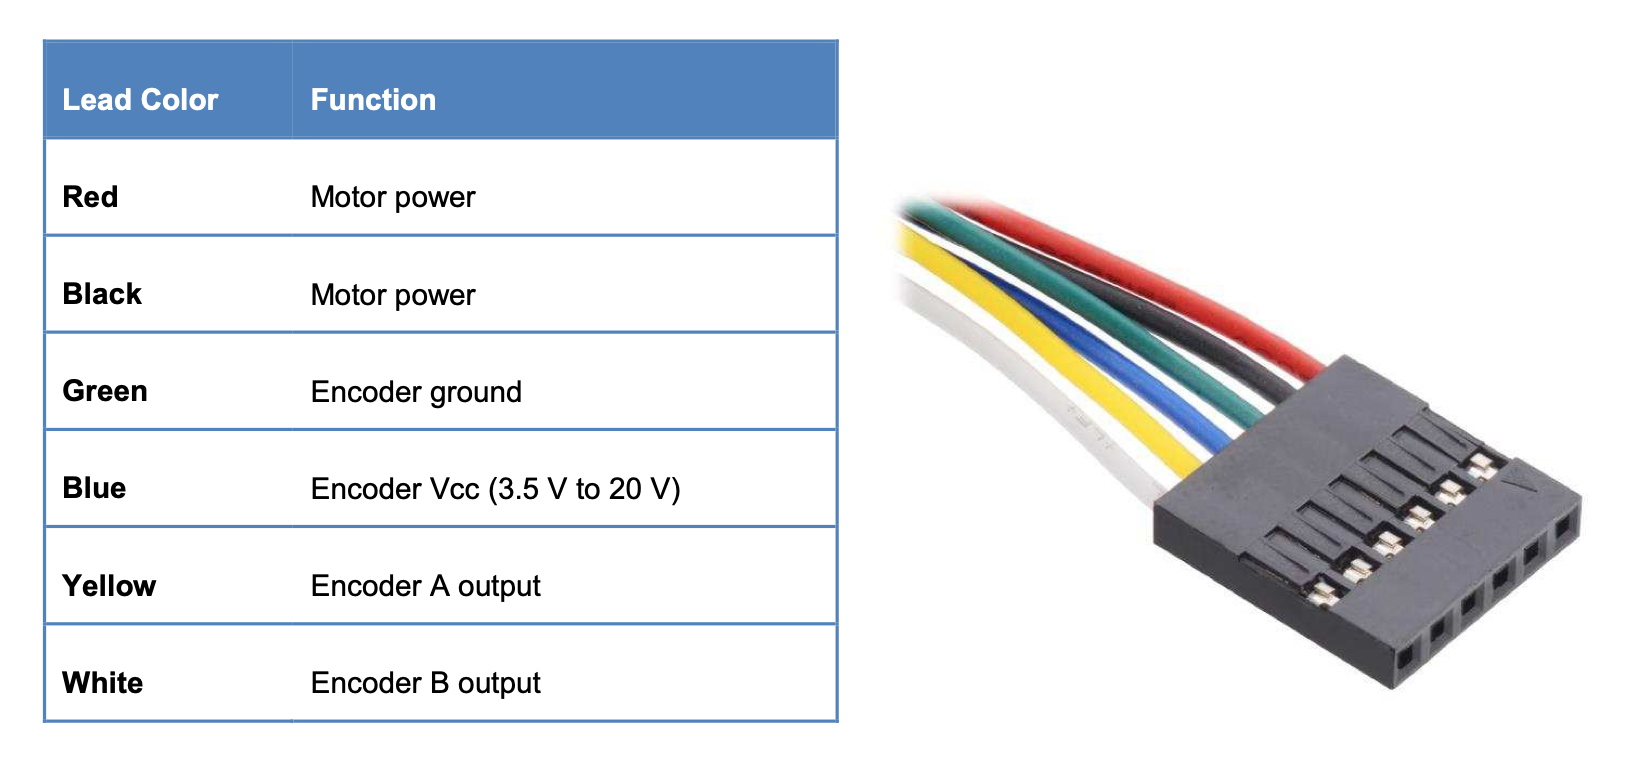
\includegraphics[width=\textwidth]{images/connector.png} 



\section{Pendulum Constants}
A multitude of other values were calculated in MATLAB.\todo{needs values for both rotors and move after rotor description}  \\

\begin{tabular}{l l}
$m$ & 0.517327 kg \\
$l$ & 0.319038 m \\
$I_{c}$ & 0.046512 kg m\textsuperscript{2} \\
$I_{f}$ & 0.000168 kg m\textsuperscript{2} \\
$g$ & 9.81 m s\textsuperscript{-2} \\
\end{tabular}




\section{Measuring Motor Constants}
\label{appendix:measure}
Measurements were made to determine a number of motor constants, including $A$, $B$, $r$, $l$, and $K_{v}$, remembering that $K_{t} = K_{v}$ provided that SI units are used.\footnote{Provided SI units are used, $K_{v}$ and $K_{t}$ will have the same magnitude.  This can be seen by equating the 
mechanical and electrical power of a motor:
\begin{equation*}
    T \omega = v i
\end{equation*}
where $T$ is the motor torque.
Rearranging,
\begin{equation*}
    \frac{T}{i} = \frac{v}{\omega}
\end{equation*}
or
\begin{equation*}
    K_{t} = K_{v} 
\end{equation*}
}
Not all of these motor constants can be directly measured.  The resistance and inductance of the motor windings can be measured with an LCR meter.
Motor voltage, current, and RPM can be measured by connecting the motor to a power supply and varying the voltage.  The RPM can be measured either with a microcontroller monitoring the encoder or using a tachometer.\\

$\frac{A}{K_{t}}$ and $\frac{B}{K_{t}}$ can be determined from \eqref{wheel} by ensuring that the motor speed is constant.  Then
\begin{equation}
    i = \frac{A}{K_{t}}sgn(\omega) + \frac{B}{K_{t}} \omega
\end{equation}
Measuring $I$ at various values of $\omega$ permits estimating both $\frac{A}{K_{t}}$ and $\frac{B}{K_{t}}$ by linear
regression.  Optimally this should be performed using the rotor mounted on the motor. This ensures that
the weight of the rotor is accurately accounted for in the gearbox friction.\\

The next step is to determine values for $K_{v}$ (and hence $K_{t}$) and $R$.  Substituting \eqref{wheel} into \eqref{motor} and assuming a constant velocity we get
\begin{equation}
    v = r\frac{A}{K_{t}}sgn(\omega) + (r\frac{B}{K_{t}}+K_{v}) \omega
\end{equation}
Knowing $\frac{A}{K_{t}}$ and $\frac{B}{K_{t}}$ from the earlier regression, $r$ and $K_{v}$ can be determined by a linear regression of $v$ as a function of $K_{v}$.  Setting $K_{t}$ equal to $K_{v}$, values for $A$ and $B$ can then be resolved.\\

Measurements of $i$, $v$, and $\omega$ were performed with the motor driven by a 12 V power supply.  Current measurements were made with a  a $\mu$Current DVM adapter and voltage measurements were 
performed at the motor input leads.  Rotor angular velocity was measured with a hand-held tachometer.  The following table list the resulting measurements:

\begin{tabular}{|c|c|c|c|cl}
\hline
Case & $v$ & $i$ & $\omega$ & $\omega$ \\
      & (V) &  (A) & (RPM) & (rad/s) \\
\hline
1	& 0.0438	& 0.0034	& 0.	& 0. \\
2	& 0.286	& 0.015	& 0.	& 0. \\
3	& 0.601	& 0.0135	& 0.	& 0. \\
4	& 0.681	& 0.0788	& 0.	& 0. \\
5	& 1.02	& 0.0591	& 80.4	& 8.42 \\
6	& 1.487	& 0.0589	& 146.	& 15.29 \\
7	& 2.012	& 0.0599	& 230.	& 24.09 \\
8	& 2.532	& 0.0631	& 307.	& 32.15 \\
9	& 3.086	& 0.065	& 386.	& 40.42 \\
10	& 3.549	& 0.067	& 454.	& 47.54 \\
11	& 3.948	& 0.0682	& 511.	& 53.51 \\
12	& 4.56	& 0.0721	& 601.	& 62.94 \\
13	& 5.03	& 0.073	& 668.	& 69.95 \\
14	& 5.94	& 0.0751	& 807.	& 84.51 \\
15	& 6.84	& 0.0751	& 940.	& 98.44 \\
16	& 7.4	& 0.0765	& 1021.	& 106.92 \\
17	& 8.44	& 0.08	& 1175.	& 123.05 \\
18	& 9.46	& 0.082	& 1323.	& 138.54 \\
19	& 10.42	& 0.0839	& 1460.	& 152.89 \\
20	& 0.2618	& 0.0354	& 0.	& 0. \\
21	& 0.3561	& 0.0481	& 0.	& 0. \\
22	& 0.476	& 0.0646	& 0.	& 0. \\
23	& 0.597	& 0.0808	& 0.	& 0. \\
24	& 0.718	& 0.0969	& 0.	& 0. \\
25	& 0.722	& 0.0543	& 49.6	& 5.19 \\
\hline
\end{tabular}

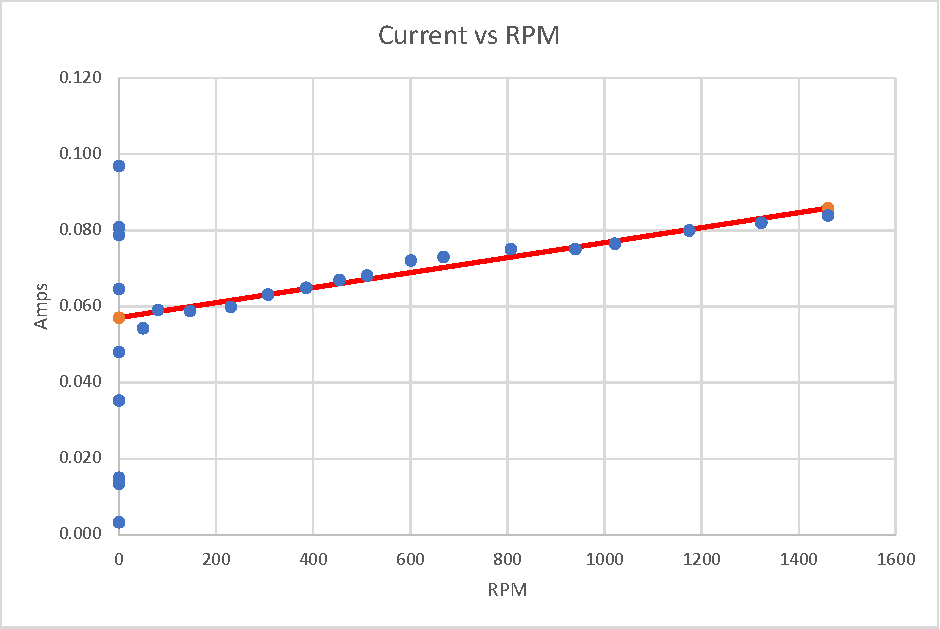
\includegraphics[width=\textwidth]{images/current.pdf} 

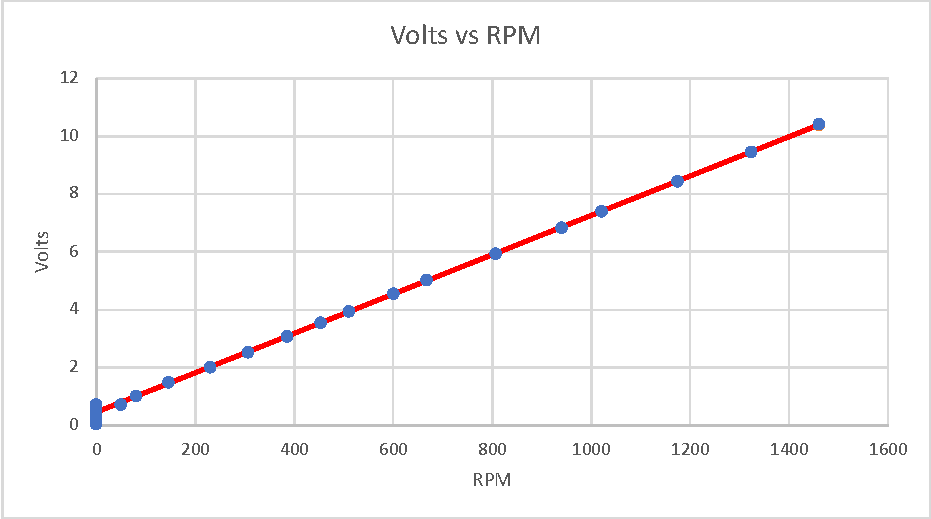
\includegraphics[width=\textwidth]{images/voltage.pdf} 


Linear regression analysis results in the following values for the motor constants:\\
$A$ = 0.00363 N m\\
$B$ = 1.2E-5 N m/(radian/sec)\\
$r$ = 7.9 $\Omega$\\
$K_{v}$ = 0.0636 V sec\\

The coulomb friction represents approximately 5\% of the 
motor stall torque.  At the motor's no-load speed the viscous friction would double the total friction to 
approximately 7\% of the motor stall torque.  The viscous friction coefficient is significantly larger than
the value of 9.06E-7 N m/(radian/sec) measured in Reference \cite{twoWheeled}.  This may be due to
the gearbox associated with the motor used in the current work.  In any event, the friction will be included
in the system modeling.\\

$l$ was 
measured with the same instrument as 6.004 mH at 1kHz.  This gives a motor electrical time constant $l/r$ of 7.6E-4 sec.  This is the time taken by the current in the motor to go from rest to 63\% of the final steady-state current.  This
validates the assumption used in  \eqref{motor} .\\



\section{Arduino Code for Measuring RPM}

The following is an Arduino sketch can be used to monitor the speed of a dc motor in lieu of a tachometer.  The sketch is designed
to work with either an Arduino Uno or an Arduino Mega. The motor wiring described in the comments
referrs to the wiring of the Pololu 25D 4.4:1 metal gear motor.  The output is in position change 
per second, where the motor has 211.2 counts/rev of gearbox shaft. \\

\lstinputlisting{../determining_motor_constants/rpm/rpm.ino}

\section{Reaction Wheel Design Options}

The initial reaction wheel design was modeled after Reference \cite{hackaday}, with modifications to allow the reaction wheel
to mate properly with a Pololu motor hub.  The reaction wheel is shown in Figure \ref{reactionWheel}.
The reaction wheel body is Aluminum 6061 with an outer diameter of 90 mm, a width of 18 mm, and an annular thickness of 7 mm. 
Fusion 360 reports the mass of the reaction wheel to be 0.09391 kg (assuming a density of 2.7 g/cc).
The moment of inertia around the centerline is 1.562E-4 kg/m2.

An alternate, simpler design (although less elegant) is shown in Figure \ref{simpleReactionWheel}.
Fashioned from carbon steel with a density of  7.85 g/cc, the diameter of the wheel is 90 mm and the
thickness is 3.175 mm (1/8").  The reaction wheel mass is 0.175 kg and the moment of inertia 
around the centerline is 1.605E-04 kg/m2.  The simpler design with only a small change in the moment
of inertia permits an easier fabrication at a cost of a doubling of the reaction wheel mass.




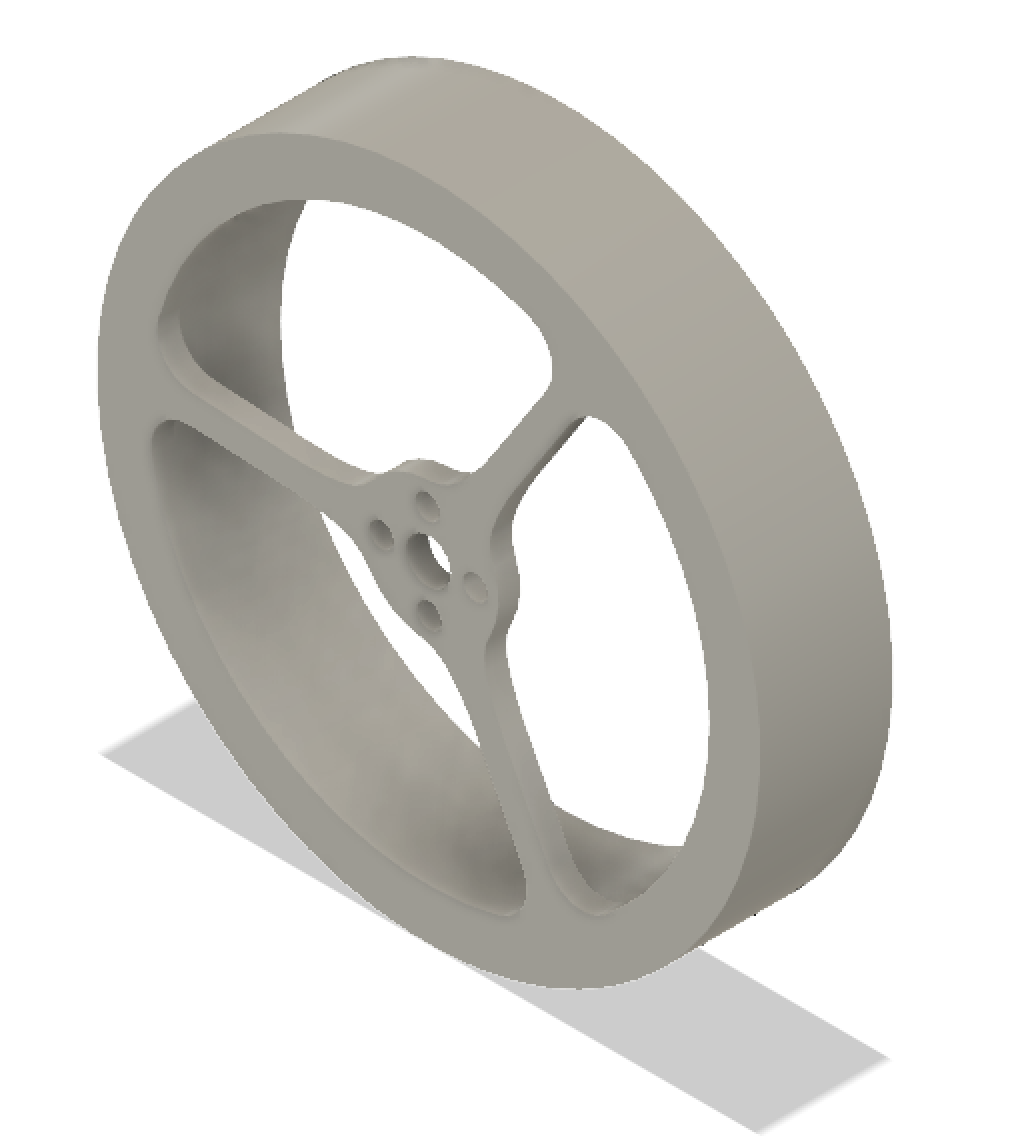
\includegraphics[width=\textwidth]{images/reactionWheel.png} 
    \captionof{figure}{Aluminum Reaction Wheel}  
    \label{reactionWheel}

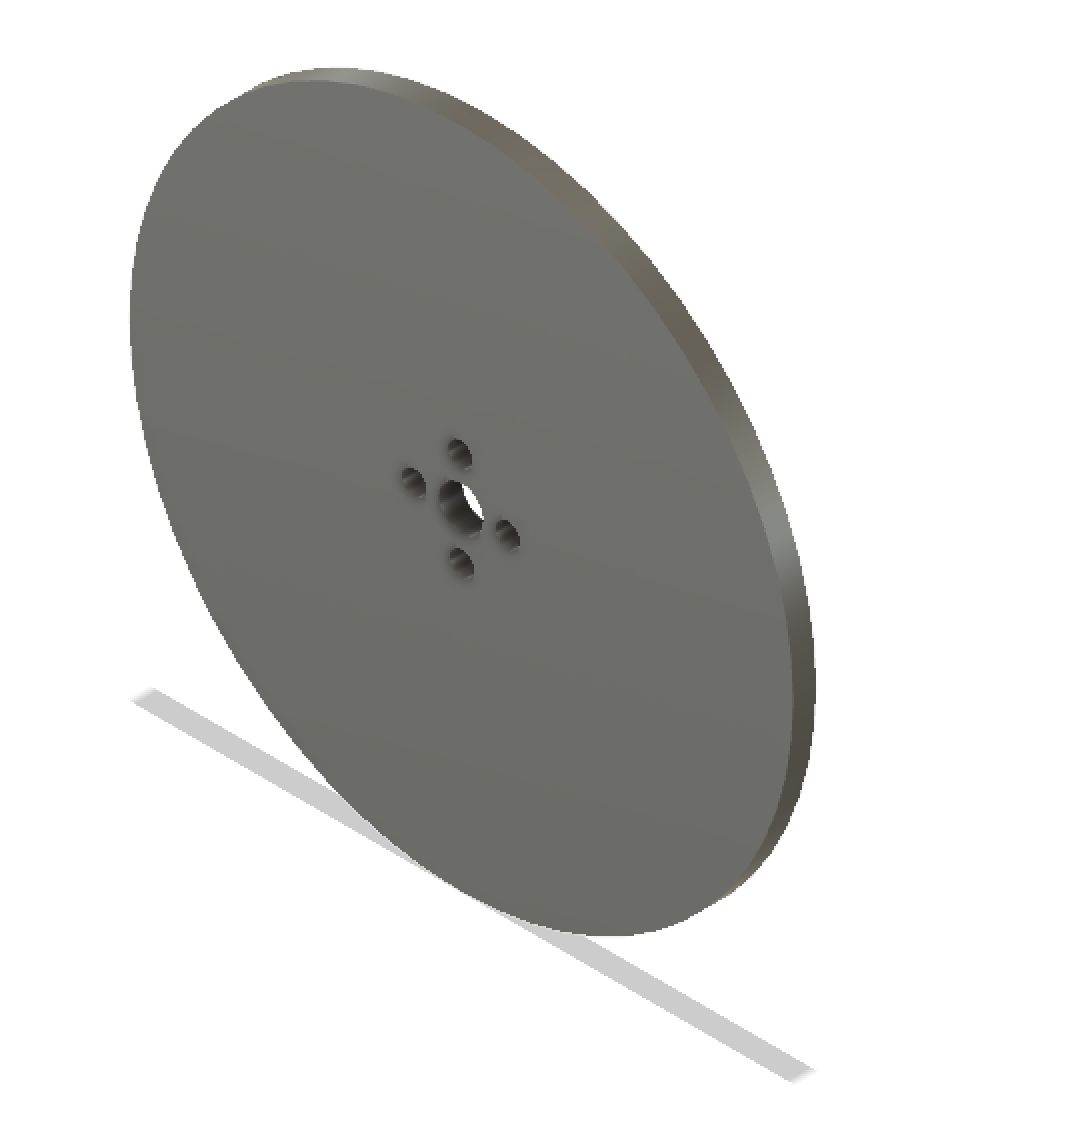
\includegraphics[width=\textwidth]{images/simpleReactionWheel.png} 
    \captionof{figure}{Simplified Carbon Steel Reaction Wheel}  
    \label{simpleReactionWheel}

\end{appendices}


\end{document}
